
\onecolumn
\begin{center}
Appendix/Supplementary Material
\end{center}
\section{Paths}\label{sec:path}
%\subsection{Zeroth Order Terms}
\textbf{Vectorised Notation:} Given a dataset $(x_s,y_s)_{s=1}^n\in \R^{d_{in}}\times \R$, let data be represented as matrices $x\in\R^{d_{in}\times n}$ and $y\in \R^n$ with the convention that $x_s=x(\cdot,s)\in\R^{d_{in}}$ and $y_s=y(s)\in \R$. For the purpose of this section we follow the vectorised notation in \Cref{tb:dgnvector}.

\FloatBarrier
\begin{table}[h]
\centering
\begin{tabular}{|c|c|}\hline
Input layer & $x(s,i,0) =x(i,s)$ \\\hline
Pre-activation& $q_t(s,i,l)= {\Theta_t(l,\cdot,i)}^\top x_t(s,\cdot,l-1) $ \\\hline
Layer output & $x_t(s,i,l)= q_t(s,i,l) G_t(s,i,l)$ \\\hline
Final output & $\hat{y}_t(x)={\Theta_t(d,\cdot,1)}^\top x_t(s,\cdot,d-1)$\\\hline
\end{tabular}
\caption{A deep gated network in the vectorised form. $l=1,\ldots,d-1$ denote the intermediate layers.}
\label{tb:dgnvector}
\end{table}




The idea behind the ``path view'' is to regard the given neural network as multitude of connections from input to output.  We now describe the zeroth and first order terms in the language of paths.
\begin{definition}[Neural Path]
Let $\P=[d_{in}]\times [w]^{d-1}$ be a cross product of index sets. Define a path $p$ by $p\stackrel{def}=(p(0),p(1),\ldots,p(d-1))\in \P$, where $p(0)\in [d_{in}]$, and $p(l)\in[w],\forall l\in[d-1]$. 
\end{definition}

A path $p$ starts at an input node $p(0)$ goes through nodes $p(l)$ in layer $l\in[d-1]$ and finishes at the output node .%(see \Cref{fig:path}%\todoch{Need to add a diagram like the recent lottery ticket weight Vivek Ramanujam paper.}). 
%In what follows, we use $p\rsa (\cdot)$ to denote the fact that path $p$ passes through node $(\cdot)$, where $(\cdot)$ is an input node, or a weight in some layer, or a hidden node.

\begin{definition}\label{def:strength}[Strength]
Each path is also associated with a strength given by: $w_t(p)=\Pi_{l=1}^d \Theta_t(l,p(l-1),p(l))$
%\begin{align}
%$w_t(p)=\Pi_{l=1}^d \Theta_t(l,p(l-1),p(l))$
%\end{align}
\end{definition}

\begin{definition}\label{def:activity}[Activation Level]
The activity of a path $p$ for input $s$ is given by: $A(s,p)=\Pi_{l=1}^d G(s,p(l),l)$
%\begin{align}
%$A(s,p)=\Pi_{l=1}^d G(s,p(l),l)$
%\end{align}
\end{definition}
In the case when $G\in \{0,1\}$ it also implies that $A\in \{0,1\}$.  %Thus $A(s,p)$ tells us whether the path $p$ is \emph{active} when $s^{th}$ input example is presented to the network.

\begin{definition}\label{def:feature}[Neural Feature]
Given a gating pattern $\G_t$, define 
\begin{align}
\phi_{x_s,\G_t}(p)\stackrel{def}=x(p(0),s) A_{\G_t}(x_s,p),
\end{align}
and let $\phi_{x_s,\G_t}=(\phi_{x_s\G_t}(p),p\in [P])\in \R^P$ be the hidden feature corresponding to input $x_s$. Let $\Phi_{x,\G_t}=\left[\phi_{x_1,\G_t}| \ldots |\phi_{x_n,\G_t}\right]\in \R^{P\times n}$ be the feature matrix obtained by stacking the features $\phi_{x_s,\G_t}$ of inputs $x_s\in \R^{d_{in}}$ column-wise.
\end{definition}

\comment{
\textbf{Predicted} output of the network is given in terms of the paths by $\hat{y}_{t}(s)=\sum_{p\in P} x(p(0),s) A_{\G_t}(x_s,p) w_t(p)$, i.e., 
\begin{align}\label{eq:zeroth}
\hat{y}_{t}(s)=\Phi_{x,\G_t}^\top w_{t}
\end{align}

%\begin{figure}
%\centering
%\includegraphics[scale=0.2]{mickey.png}
%\caption{Some picture to break the monotony}
%\end{figure}

%\textbf{Sub-networks:} %An important fact that can be seen as an immediately from the path based representation is that DGNs 
\textbf{Sub-networks:}  In DGNs similarity of two different inputs $x_s,x_{s'}\in \R^{d_{in}}, s,s' \in [n]$ depends on the overlap of path that are \emph{active} for both inputs. This can be seen by noting that $\phi_{x_s,\G_t}^\top \phi_{x_s,\G_t}=\sum_{i=1}^{d_{in}} x(i,s)x(i,s') \underset{p\rsa i}{\sum} A_{\G_t}(x_s,p) A_{\G_t}(x_{s'},p)$. Consider for instance a DGN whose gating values are in $\{0,1\}$, and say $n=2$, i.e., the dataset contains only two inputs $x_1,x_2\in \R^{d_{in}}$. From \eqref{eq:pathsim} it is clear that if inputs $x_1,x_2$ do not share any common \emph{active} paths throughout training, then they are \emph{orthogonal} to each other, because $A_{\G_t}(s,p) A_{\G_t}(s',p)=0, \forall p\in [P]$. This makes intuitive sense because in this case, it is as though there are two parallel networks (while the weights can be shared, the paths are not). Thus it is clear from the path based representation in \eqref{eq:zeroth} and \eqref{eq:pathsim}, the gating pattern $\G_t$ plays are crucial role in DGNs via the activation levels $A_{\G_t}(\cdot,\cdot)$.
%\subsection{First Order Terms}
The feature $\phi_{x_s,\G_t}$ in \Cref{def:feature} as well as the strength $w_t$ in \Cref{def:strength} are $P$-dimensional quantities. However, loosely speaking, the DGN has only as much \emph{degrees of freedom} as the number of trainable parameters (which we denote by $d_{net}$). 
\begin{definition}[Neural Tangent Features] The  $d_{net}\times n$ NTF matrix is defined as $\Psi_t(m,s)\stackrel{def}=\frac{\partial \hat{y}_{t}(x_s)}{\partial \theta(m)},m\in [d_{net}], s\in [n]$. 
\comment{
\begin{align}\label{eq:split}
\begin{split}
&\Psi_t(m,s) = \frac{\partial \hat{y}_t(x_s)}{\partial \theta(m)}\\
&=\frac{\partial }{\partial \theta(m)}\left(\sum_{p\in P} x(p(0),s) w_{t}(p) A_{\G_t}(s,p)\right),\\
&=\underbrace{\left(\sum_{p\in P} x(p(0),s) \frac{\partial w_{t}(p)}{\partial \theta(m)} A_{\G_t}(s,p)\right)}_{\text{sensitivity of strength}}\\
&\quad\quad\quad\quad\quad\quad\quad\quad+\\
&=\underbrace{\left(\sum_{p\in P} x(p(0),s) w_{t}(p) \frac{\partial A_{\G_t}(s,p)}{\partial \theta(m)}\right)}_{\text{sensitivity of activations}}
\end{split}
\end{align}

\begin{align}\label{eq:split}
\begin{split}
&\Psi_t(m,s) = \frac{\partial \hat{y}_t(x_s)}{\partial \theta(m)}\\
&=\frac{\partial }{\partial \theta(m)}\left(\sum_{p\in P} x(p(0),s) w_{t}(p) A_{\G_t}(s,p)\right),\\
&=\underbrace{\left(\sum_{p\in P} x(p(0),s) \frac{\partial w_{t}(p)}{\partial \theta(m)} A_{\G_t}(s,p)\right)}_{{\Psi^w_{t}(m,s)}}\\
&\quad\quad\quad\quad\quad\quad\quad\quad+\\
&=\underbrace{\left(\sum_{p\in P} x(p(0),s) w_{t}(p) \frac{\partial A_{\G_t}(s,p)}{\partial \theta(m)}\right)}_{{\Psi^a_t(m,s)}}
\end{split}
\end{align}
}
\comment{
\begin{align}\label{eq:split}
\begin{split}
\Psi_t(m,s) &= \underbrace{\left(\sum_{p\in P} x(p(0),s) \frac{\partial w_{t}(p)}{\partial \theta(m)} A_{\G_t}(s,p)\right)}_{{\Psi^w_{t}(m,s)}}\\
&\quad\quad\quad\quad\quad\quad\quad\quad+\\
&=\underbrace{\left(\sum_{p\in P} x(p(0),s) w_{t}(p) \frac{\partial A_{\G_t}(s,p)}{\partial \theta(m)}\right)}_{{\Psi^a_t(m,s)}}
\end{split}
}
\begin{align}\label{eq:split}
\begin{split}
\Psi_t(m,s) &= \Psi^w_{t}(m,s)+\Psi^a_{t}(m,s), \,\text{where}\\
\Psi^w_{t}(m,s)&={\left(\sum_{p\in P} x(p(0),s) \frac{\partial w_{t}(p)}{\partial \theta(m)} A_{\G_t}(s,p)\right)}\\
\Psi^a_{t}(m,s)&={\left(\sum_{p\in P} x(p(0),s) w_{t}(p) \frac{\partial A_{\G_t}(s,p)}{\partial \theta(m)}\right)}
\end{split}
\end{align}


\end{definition}

\textbf{Strength and Gate adaptation:} From \eqref{eq:split} it is clear that there are two \emph{atomic} components to the gradient of the output $\hat{y}_t(x_s)$ with respect to any trainable weight $\theta(m), m=1,\ldots, d_{net}$, namely \emph{neural tangent feature of strength} denoted by $\Psi^w_{t}\in \R^{d_{net}\times n}$ and \emph{neural tangent feature of activations} denoted by $\Psi^a_{t}\in \R^{d_{net}\times n}$. %Before we separately define these two \emph{atomic} components, we would like to mention that as a result of the $\frac{\partial A_{\G_t}(s,p)}{\partial \theta(m)}$ term, gates adapt all throughout training, which in turn affect the output (see \eqref{eq:zeroth}) via $A_{\G_t}$.

}


\comment{
\begin{definition}[Neural Tangent Features of Path Activations (NTFPA)]
\begin{align}
\varphi^a_{t,p}\stackrel{def}{=}\left(\frac{\partial w_{t}(p)}{\partial \theta(m)},m\in[d_{net}]\right)\in \R^{d_{net}},
\end{align}
\end{definition}

\begin{remark}
Let $\theta(m)$ belong to layer $l'\in [d-1]$, then 
\begin{align*}
\varphi^a_{t,p}(m)&=0, \forall p\bcancel{\rsa}\theta(m)
\end{align*}
\end{remark}

Using the sensitivity of strengths and activations at the level of resolution of paths, we now define the neural tangent feature (NTF) for the strengths and activations.

\begin{definition}\label{def:ntf}[Neural Tangent Features]
\begin{align}
\begin{split}
\Psi^w_t(m,s) &=\left(\sum_{p\in P} x(p(0),s) \frac{\partial w_{t}(p)}{\partial \theta(m)} A_{\G_t}(s,p)\right)\\
\Psi^a_t(m,s) &=\left(\sum_{p\in P} x(p(0),s) w_{t}(p) \frac{\partial A_{\G_t}(s,p)}{\partial \theta(m)}\right)\\
\Psi_t(m,s)&=\Psi^w_t(m,s)+ \Psi^a_t(m,s)
\end{split}
\end{align}
\end{definition}


\begin{definition}[Interaction Coefficient]
\begin{align*}
&\lambda^{s,s'}_t(i)\stackrel{def}=\underset{p_1,p_2\rsa\theta(m),i}{\sum_{p_1,p_2\in P:}}  \varphi_{t,p_1}(m)A(s,p_1)  \varphi_{t,p_2}(m) A(s',p_2)
\end{align*}
\end{definition}

\begin{lemma}
\begin{align*}
{K^w_t(s,s')}=\sum_{i=1}^{d_{in}} x(i,s)x(i,s') \lambda^{s,s'}_t(i)
\end{align*}
\end{lemma}

\begin{assumption}\label{assmp:main}\hfill
\begin{enumerate}
\item $\G_0$ is statistically independent of $\Theta_0$.
\item $\Theta_0\stackrel{iid}\sim Ber(\frac{1}{2})$ over the set $\{-\sigma,+\sigma\}$. 
\end{enumerate}
\end{assumption}

\textbf{Remarks on Assumption~\ref{assmp:main}}
In a standard DNN with ReLU activations, the activations and weights are not statistically independent because conditioned on the fact that a ReLU is \emph{on}, the incoming edges cannot be simultaneously all $-\sigma$. We side step this issue by the first condition in Assumption~\ref{assmp:main}, wherein, we assume that  gating is statistically independent of the weights $\Theta_0$. This clears the way to carry out the algebra of paths, which can be boiled down in simple words as the effect on weights in the direction of one path does not affect the contribution of any other path in expectation. This is captured in Lemma~\ref{lm:pathdot} below.
\begin{figure}
\centering
\includegraphics[scale=0.2]{mickey.png}
\caption{Shows that the incoming weights of a ReLU gate which are \emph{on} are not symmetrically distributed.}
\end{figure}

\begin{lemma}\label{lm:pathdot}
Let $\theta(m)$ be an arbitrary weight in layer $l'\in [d-1]$, under Assumption~\ref{assmp:init} we have for paths $p,p_1,p_2\rsa\theta(m), p_1\neq p_2$
\begin{align*}
\E{\varphi_{\Tb,p_1}(m)\varphi_{\Tb,p_2}(m)}= &0\\
\E{\varphi_{\Tb,p}(m)\varphi_{\Tb,p}(m)}= &\left(\frac{2\sigma^2}{w}\right)^{d-1}
\end{align*}
\end{lemma}
\begin{proof}
If $\theta$
Note that $\varphi_{\Tb,p}=\underset{l\neq l'}{\underset{l=1}{\overset{d}{\Pi}}} \Tb(l,p(l-1),p(l))$. Hence
\begin{align*}
&\E{\varphi_{\Tb,p_1}(m)\varphi_{\Tb,p_2}(m)}\\
&=\E{\underset{l\neq l'}{\underset{l=1}{\overset{d}{\Pi}}} \Bigg(\Tb(l,p_1(l-1),p_1(l))\Tb(l,p_2(l-1),p_2(l)) \Bigg)}\\
&=\underset{l\neq l'}{\underset{l=1}{\overset{d}{\Pi}}}\E{\Tb(l,p_1(l-1),p_1(l))\Tb(l,p_2(l-1),p_2(l))}
\end{align*}

Since $p_1\neq p_2$, in one of the layers $\tilde{l}\in[d-1],\tilde{l}\neq l'$ they do not pass through the same weight. Using this fact
\begin{align*}
&\E{\varphi_{\Tb,p_1}(m)\varphi_{\Tb,p_2}(m)}\\
&=\left(\underset{l\neq l',\tilde{l}}{\underset{l=1}{\overset{d}{\Pi}}}\E{\Tb(l,p_1(l-1),p_1(l))\Tb(l,p_2(l-1),p_2(l))}\right)\\
&\Bigg(\E{\Tb(\tilde{l},p_1(\tilde{l}-1),p_1(\tilde{l}))}\E{\Tb(\tilde{l},p_2(\tilde{l}-1),p_2(\tilde{l}))}\Bigg)\\
&=0
\end{align*}
\end{proof}


\begin{definition}[Path Similarity]
\begin{align*}
\mu^{s,s'}(i)=\sum_{m=1}^{d_{net}} \underset{p\rsa\theta(m)}{\sum_{p\in P: p(0)=i}}A(s,p) A(s',p)
\end{align*}

\end{definition}

\begin{lemma}
\begin{align*}
\mathbf{E}_{\Theta_0}\left[\lambda^{s,s'}_0(i)\right]=\sigma^{2(d-1)}\mu^{s,s'}(i)
\end{align*}
\end{lemma}

\begin{theorem}\label{th:dgnexp}
 Under Assumption~\ref{assmp:main}
 \begin{align*}
\mathbf{E}_{\Theta_0}\left[K_0(s,s')\right]=\sigma^{2(d-1)}\sum_{i=1}^{d_{in}}x(i,s) x(i,s')\mu^{s,s'}(i)
\end{align*}

\end{theorem}
\begin{proof}
See Appendix.
\end{proof}

\begin{theorem}\label{th:dgnvar}
 Under Assumption~\ref{assmp:main} $Var\left[K_0\right]\leq $
\end{theorem}

}
% This document was modified from the file originally made available by
% Pat Langley and Andrea Danyluk for ICML-2K. This version was created
% by Iain Murray in 2018, and modified by Alexandre Bouchard in
% 2019. Previous contributors include Dan Roy, Lise Getoor and Tobias
% Scheffer, which was slightly modified from the 2010 version by
% Thorsten Joachims & Johannes Fuernkranz, slightly modified from the
% 2009 version by Kiri Wagstaff and Sam Roweis's 2008 version, which is
% slightly modified from Prasad Tadepalli's 2007 version which is a
% lightly changed version of the previous year's version by Andrew
% Moore, which was in turn edited from those of Kristian Kersting and
% Codrina Lauth. Alex Smola contributed to the algorithmic style files.

\subsection{Results in \Cref{sec:optimisation}}
\textbf{Stament and Proof of Lemma~\ref{lm:sigwire}}
\begin{lemma}[Signal vs Wire Decomposition]
Let $\kappa_t(s,s',i)\stackrel{def}=\underset{p_1,p_2\rsa i}{\sum_{p_1,p_2\in P:}} A_{\G_t}(x_s,p_1) A_{\G_t}(x_{s'},p_2) \ip{\varphi_{t,p_1}, \varphi_{t,p_2}}$. The Gram matrix $K_t$ is then given by 
\begin{align}\label{eq:ktalg}
{K_t(s,s')}=\sum_{i=1}^{d_{in}} x(i,s)x(i,s') \kappa_t(s,s',i)
\end{align}
\end{lemma}

\begin{proof}
Note that
\begin{align*}
\hat{y}_{t}(x_s)=\sum_{p\in\P}x(p(0),s) A(x_s,p) w_t(p)
\end{align*}
Differentiating with respect to any of the weights $\theta(m),m\in[d_{net}]$, we have
\begin{align*}
\frac{\partial \hat{y}_{t}(x_s)}{\partial \theta(m)}&=\frac{\partial \sum_{p\in\P}x(p(0),s) A(x_s,p) w_t(p)}{\partial \theta(m)}\\
\Psi_t(m,s)&=\sum_{p\in\P}x(p(0),s) A(x_s,p) \frac{\partial w_t(p)}{\partial \theta(m)}\\
&=\sum_{p\in\P}x(p(0),s) A(x_s,p) \varphi_{t,p}(m)
\end{align*}

Since, only the path strengths are changing, the Gram matrix $K_t$ is given by 
\begin{align*}
K_t(s,s')&={\Psi_t(\cdot,s)}^\top \Psi_t(\cdot,s')\\
&=\sum_{m=1}^{d_{net}} \Psi_t(m,s) \Psi_t(m,s')\\
&=\sum_{m=1}^{d_{net}} \left(\sum_{p_1\in\P}x(p_1(0),s) A(x_s,p_1) \varphi_{t,p_1}(m)\right)\left(\sum_{p_2\in\P}x(p_2(0),s') A(x_{s'},p_2) \varphi_{t,p_2}(m)\right)\\
&=\sum_{m=1}^{d_{net}} \underset{p_1,p_2\rsa\theta(m)}{\sum_{p_1,p_2\in P:}} x(p_1(0),s) A(x_s,p_1)x(p_2(0),s') A(x_{s'},p_2) \varphi_{t,p_1}(m) \varphi_{t,p_2}(m)\\
&=\sum_{i=1}^{d_{in}}\underset{p_1,p_2\rsa i}{\sum_{p_1,p_2\in P:}} x(p_1(0),s) A(x_s,p_1)x(p_2(0),s') A(x_{s'},p_2) \ip{\varphi_{t,p_1}, \varphi_{t,p_2}}\\
&=\sum_{i=1}^{d_{in}}\underset{p_1,p_2\rsa i}{\sum_{p_1,p_2\in P:}} x(i,s) A(x_s,p_1)x(i,s') A(x_{s'},p_2) \ip{\varphi_{t,p_1}, \varphi_{t,p_2}}\\
&=\sum_{i=1}^{d_{in}} x(i,s)x(i,s') \underset{p_1,p_2\rsa i}{\sum_{p_1,p_2\in P:}} A(x_s,p_1) A(x_{s'},p_2) \ip{\varphi_{t,p_1}, \varphi_{t,p_2}}
\end{align*}
\end{proof}


\textbf{Statement and Proof of Lemma~\ref{lm:pathdot}}
\begin{lemma}
Under Assumption~\ref{assmp:mainone}, for paths $p,p_1,p_2\in \P, p_1\neq p_2$, at initialisation we have (i) $\E{\ip{\varphi_{0,p_1}, \varphi_{0,p_2}}}= 0$, (ii) ${\ip{\varphi_{0,p}, \varphi_{0,p}}}= d\sigma^{2(d-1)}$
\end{lemma}

\begin{proof}
\begin{align*}
\ip{\varphi_{t,p_1}, \varphi_{t,p_2}}= \sum_{m=1}^{d_{net}} \varphi_{t,p_1}(m)\varphi_{t,p_2}(m)
\end{align*}
Let $\theta(m),m\in[d_{net}]$ be any weight such that $p\rsa \theta(m)$, and w.l.o.g let $\theta(m)$ belong to layer $l'\in[d]$. 
If either $p_1\bcancel{\rsa}\theta(m)$ or $p_2\bcancel{\rsa}\theta(m)$, then it follows that $\varphi_{t,p_1}(m)\varphi_{t,p_2}(m)=0$. In the case when $p_1,p_2\rsa\theta(m)$, we have
\begin{align*}
&\E{\varphi_{0,p_1}(m)\varphi_{0,p_2}(m)}\\
&=\E{\underset{l\neq l'}{\underset{l=1}{\overset{d}{\Pi}}} \Bigg(\Tb_0(l,p_1(l-1),p_1(l))\Tb_0(l,p_2(l-1),p_2(l)) \Bigg)}\\
&=\underset{l\neq l'}{\underset{l=1}{\overset{d}{\Pi}}}\E{\Tb_0(l,p_1(l-1),p_1(l))\Tb_0(l,p_2(l-1),p_2(l))}
\end{align*}
where the $\E{\cdot}$ moved inside the product because at initialisation the weights (of different layers) are independent of each other.
Since $p_1\neq p_2$, in one of the layers $\tilde{l}\in[d-1],\tilde{l}\neq l'$ they do not pass through the same weight, i.e., $\Tb_0(\tilde{l},p_1(\tilde{l}-1),p_1(\tilde{l}))$ and $\Tb_0(\tilde{l},p_2(\tilde{l}-1),p_2(\tilde{l}))$ are distinct weights. Using this fact
\begin{align*}
&\E{\varphi_{0,p_1}(m)\varphi_{0,p_2}(m)}\\
&=\underset{l\neq l',\tilde{l}}{\underset{l=1}{\overset{d}{\Pi}}}\E{\Tb_0(l,p_1(l-1),p_1(l))\Tb_0(l,p_2(l-1),p_2(l))}\\
&=\E{\Tb_0(\tilde{l},p_1(\tilde{l}-1),p_1(\tilde{l}))}\E{\Tb_0(\tilde{l},p_2(\tilde{l}-1),p_2(\tilde{l}))}\\
&=0
\end{align*}

The proof of (ii) is complete by noting that $\sum_{m=1}^{d_{net}} \varphi_{t,p}(m)\varphi_{t,p}(m)$ has $d$ non-zero terms for a single path $p$ and at initialisation we have 
\begin{align*}
&{\varphi_{0,p}(m)\varphi_{0,p}(m)}\\
&={\underset{l\neq l'}{\underset{l=1}{\overset{d}{\Pi}}} \Tb^2_0(l,p(l-1),p(l))}\\
&=\sigma^{2(d-1)}
\end{align*}
\end{proof}

\textbf{Statement and Proof of Theorem~\ref{th:dgnexp}}
\begin{theorem}[DIP in DGN]
Under Assumption~\ref{assmp:mainone}, ~\ref{assmp:maintwo}, and $\frac{4d}{w^2}<1$ it follows that
 \begin{align*}
&\E{K_0}=d\sigma^{2(d-1)}(x^\top x \odot \lambda_0)\\
&Var\left[K_0\right]\leq O\left(d^2_{in}\sigma^{4(d-1)}\max\{d^2w^{2(d-2)+1}, d^3w^{2(d-2)}\}\right)
\end{align*}
\end{theorem}

\begin{proof}
The first of the above two claims follow from the algebraic expression for $K_t$ and Lemma~\ref{lm:pathdot}. We now look at the variance calculation. The idea is that we expand  $Var\left[K_0(s,s')\right]=\E{K_0(s,s')^2} -\E{K_0(s,s')}^2$ and identify the the terms which cancel due to subtraction and then bound the rest of the terms.% Further, in what follows, we will assume $d_{in}=1$ without loss of generality.

Let $\theta(m)$ belong to layer $l'(m)$, then 
\begin{align}\label{eq:kexpect}
\E{K_0(s,s')}&=\sum_{m=1}^{d_{net}}\E{\left(\sum_{p_1 \in P}x(p_1(0),s)A(s,p_1)\frac{\partial w_{\Tb}(p_1)}{\partial \theta(m)}\right)\left(\sum_{p_2\in P}x(p_2(0),s)A(s',p_2)\frac{\partial w_{\Tb}(p_2)}{\partial \theta(m)}\right)}\nn\\
&=\sum_{m=1}^{d_{net}}\E{\sum_{p_1,p_2\in P}x(p_1(0),s)A(s,p_1)\frac{\partial w_{\Tb}(p_1)}{\partial \theta(m)}x(p_2(0),s')A(s',p_2)\frac{\partial w_{\Tb}(p_2)}{\partial \theta(m)}}\nn\\
&=\sum_{m=1}^{d_{net}}\underset{p_1,p_2\rsa\theta(m)}{\sum_{p_1,p_2\in P}}x(p_1(0),s)A(s,p_1)x(p_2(0),s')A(s',p_2) \E{\underset{l\neq l'(m)}{\underset{l=1}{\overset{d-1}{\Pi}}} \Tb_0(l,p_1(l-1),p_1(l)) \Tb_0(l,p_2(l-1),p_2(l))}\nn\\
&\stackrel{(a)}=\sum_{m=1}^{d_{net}}\underset{p_1,p_2\rsa\theta(m)}{\sum_{p_1,p_2\in P}}x(p_1(0),s)A(s,p_1)x(p_2(0),s')A(s',p_2) \underset{l\neq l'(m)}{\underset{l=1}{\overset{d-1}{\Pi}}} \E{\Tb_0(l,p_1(l-1),p_1(l)) \Tb_0(l,p_2(l-1),p_2(l))}
\end{align}
where $(a)$ follows from the fact that at initialisation the layer weights are independent of each other. Note that the right hand side of \eqref{eq:kexpect} only terms with $p_1=p_2$ will survive the expectation.

In the expression in \eqref{eq:kexpectsquare} note that $p_1=p_2$ and $p_3=p_4$.
\begin{align}\label{eq:kexpectsquare}
&\E{K_0(s,s')}^2=\nn\\
&\left(\sum_{m=1}^{d_{net}}\underset{p_1,p_2\rsa\theta(m)}{\sum_{p_1,p_2\in P}}x(p_1(0),s)A(s,p_1)x(p_2(0),s')A(s',p_2) \underset{l\neq l'(m)}{\underset{l=1}{\overset{d-1}{\Pi}}} \E{\Tb_0(l,p_1(l-1),p_1(l)) \Tb_0(l,p_2(l-1),p_2(l))}\right)\nn\\
&\left(\sum_{m'=1}^{d_{net}}\underset{p_3,p_4\rsa\theta(m')}{\sum_{p_3,p_4\in P}}x(p_3(0),s)A(s,p_3)x(p_4(0),s')A(s',p_4) \underset{l\neq l'(m')}{\underset{l=1}{\overset{d-1}{\Pi}}} \E{\Tb_0(l,p_3(l-1),p_3(l)) \Tb_0(l,p_4(l-1),p_4(l))}\right)\nn\\
&=\nn\\
&\sum_{m,m'=1}^{d_{net}}\underset{p_3,p_4\rsa\theta(m')}{\underset{p_1,p_2\rsa\theta(m)}{\sum_{p_1,p_2,p_3,p_4\in P}}}\Bigg[\bigg(x(p_1(0),s)A(s,p_1)x(p_2(0),s')A(s',p_2)x(p_3(0),s)A(s,p_3)x(p_4(0),s')A(s',p_4)\bigg)\nn\\
&\bigg( \underset{l\neq l'(m)} {\underset{l\neq l'(m')}{\underset{l=1}{\overset{d-1}{\Pi}}}} \E{\Tb_0(l,p_1(l-1),p_1(l)) \Tb_0(l,p_2(l-1),p_2(l))}\E{\Tb_0(l,p_3(l-1),p_3(l)) \Tb_0(l,p_4(l-1),p_4(l))} \bigg)\nn\\
&\bigg( \E{\Tb_0(l,p_1(l'(m')-1),p_1(l'(m'))) \Tb_0(l,p_2(l'(m')-1),p_2(l'(m')))}\bigg)\nn\\
&\bigg(\E{\Tb_0(l,p_3(l'(m)-1),p_3(l'(m))) \Tb_0(l,p_4(l'(m)-1),p_4(l'(m)))} \bigg)\Bigg]\nn\\
\end{align}

In the expression in \eqref{eq:ksquareexpect}, paths $p_1,p_2,p_3,p_4$ do not have constraints, and can be distinct.
\begin{align}\label{eq:ksquareexpect}
&\E{K^2_0(s,s')}=\nn\\
&\sum_{m,m'=1}^{d_{net}}\underset{p_3,p_4\rsa\theta(m')}{\underset{p_1,p_2\rsa\theta(m)}{\sum_{p_1,p_2,p_3,p_4\in P}}}\Bigg[\bigg(x(p_1(0),s)A(s,p_1)x(p_2(0),s')A(s',p_2)x(p_3(0),s)A(s,p_3)x(p_4(0),s')A(s',p_4)\bigg)\nn\\
&\bigg( \underset{l\neq l'(m)} {\underset{l\neq l'(m')}{\underset{l=1}{\overset{d-1}{\Pi}}}} \E{\Tb_0(l,p_1(l-1),p_1(l)) \Tb_0(l,p_2(l-1),p_2(l))\Tb_0(l,p_3(l-1),p_3(l)) \Tb_0(l,p_4(l-1),p_4(l))} \bigg)\nn\\
&\bigg( \E{\Tb_0(l,p_1(l'(m')-1),p_1(l'(m'))) \Tb_0(l,p_2(l'(m')-1),p_2(l'(m')))}\bigg)\nn\\
&\bigg(\E{\Tb_0(l,p_3(l'(m)-1),p_3(l'(m))) \Tb_0(l,p_4(l'(m)-1),p_4(l'(m)))} \bigg)\Bigg]\nn\\
\end{align}

We now state the following facts/observations.

$\bullet$ \textbf{Fact 1:} Any term that survives the expectation (i.e., does not become $0$) and participates in \eqref{eq:ksquareexpect} is of the form $\sigma^{4(d-1)}\big(x(p_1(0),s)A(s,p_1)x(p_2(0),s')A(s',p_2)x(p_3(0),s)A(s,p_3)x(p_4(0),s')A(s',p_4)\big)$, where $p_1,p_2,p_3,p_4$ are free variables, and participates in \eqref{eq:kexpectsquare} is of the form $\sigma^{4(d-1)}\big(x(p_1(0),s)A(s,p_1)x(p_2(0),s')A(s',p_2)x(p_3(0),s)A(s,p_3)x(p_4(0),s')A(s',p_4)\big)$, where $p_1=p_2,p_3=p_4$.

$\bullet$ \textbf{Fact 2:} The number of paths through a particular weight $\theta(m)$ in one of the middle layers is $d_{in}w^{d-3}$, and the number of paths through a particular weight $\theta(m)$ in either the first or the last layer is $d_{in}w^{d-2}$ .

$\bullet$ \textbf{Fact 3:} Let $\P'$ be an arbitrary set of paths constrained to pass through some set of weights. Let $\P''$ be the set of paths obtained by adding an additional constraint that the paths also should pass through a particular weight say $\theta(m)$. Now, if $\theta(m)$ belongs to :

$1.$ a middle layer, then $|\P''|=\frac{|\P'|}{w^2}$.

$2.$ the first layer or the last layer, then $|\P''|=\frac{|\P'|}{w}$.

$\bullet$ \textbf{Fact 4:} For any $p_1,p_2,p_3,p_4$ combination that survives the expectation in \eqref{eq:ksquareexpect} can be written as 

\begin{align*}
&\bigg( \underset{l\neq l'(m)} {\underset{l\neq l'(m')}{\underset{l=1}{\overset{d-1}{\Pi}}}} \E{\Tb_0(l,p_1(l-1),p_1(l)) \Tb_0(l,p_2(l-1),p_2(l))\Tb_0(l,p_3(l-1),p_3(l)) \Tb_0(l,p_4(l-1),p_4(l))} \bigg)\nn\\
&\bigg( \E{\Tb_0(l,p_1(l'(m')-1),p_1(l'(m'))) \Tb_0(l,p_2(l'(m')-1),p_2(l'(m')))}\bigg)\nn\\
&\bigg(\E{\Tb_0(l,p_3(l'(m)-1),p_3(l'(m))) \Tb_0(l,p_4(l'(m)-1),p_4(l'(m)))} \bigg)\Bigg]\nn\\
&=\\
&\bigg( \underset{l\neq l'(m)} {\underset{l\neq l'(m')}{\underset{l=1}{\overset{d-1}{\Pi}}}} \Tb^2_0(l,\rho_a(l-1),\rho_a(l)) \Tb^2_0(l,\rho_b(l-1),\rho_b(l)) \bigg)\nn\\
&\bigg( \Tb^2_0(l,\rho_a(l'(m')-1),\rho_a(l'(m')))\bigg)\nn\\
&\bigg({\Tb^2_0(l,\rho_b(l'(m)-1),\rho_b(l'(m)))} \bigg),
\end{align*}

where $\rho_a\rsa \theta(m)$ and $\rho_b\rsa \theta(m')$ are what we call as \emph{base} (case) paths. 


$\bullet$ \textbf{Fact 5:} For any given base paths $\rho_a$ and $\rho_b$ there could be multiple assignments possible for $p_1,p_2,p_3,p_4$.

$\bullet$ \textbf{Fact 6:}  Terms in \eqref{eq:ksquareexpect}, wherein, the base case is generated as $p_1=p_2=\rho_a$ and $p_3=p_4=\rho_b$ (or $p_1=p_2=\rho_b$ and $p_3=p_4=\rho_a$), get cancelled with the corresponding terms in \eqref{eq:kexpectsquare}.

$\bullet$ \textbf{Fact 7:}  When the bases paths $\rho_a$ and $\rho_b$ do not intersect (i.e., do not pass through the same weight in any one of the layers), the only possible assignment is $p_1=p_2=\rho_a$ and $p_3=p_4=\rho_b$ (or $p_1=p_2=\rho_b$ and $p_3=p_4=\rho_a$), and such terms are common in \eqref{eq:ksquareexpect} and \eqref{eq:kexpectsquare}, and hence do not show up in the variance term.


$\bullet$ \textbf{Fact 7:} Let base paths $\rho_a$ and $\rho_b$ cross at layer $l_1, \ldots, l_k, k \in [d-1]$, and let $\rho_a=(\rho_a(1),\ldots,\rho_a(k+1))$ where $\rho_a(1)$ is a sub-path string from layer $1$ to $l_1$, and $\rho_a(2)$ is the sub-path string from layer $l_1+1$ to $l_2$ and so on, and $\rho_a(k+1)$ is the sub-path string from layer $l_k+1$ to the output node. Then the set of paths that can occur in $\E{K_0(s,s')^2}$ are of the form:
\begin{enumerate}
\item $p_1=p_2=\rho_a, p_3=p_4=\rho_b$ (or $p_1=p_2=\rho_b, p_3=p_4=\rho_a$) which get cancelled in the $\E{K_0(s,s')}^2$ term.
\item $p_1=\rho_a$, $p_3=\rho_b$, $p_2=(\rho_b(1),\rho_a(2),\rho_a(3),\ldots,\rho_a(k+1))$, $p_4=(\rho_a(1),\rho_b(2),\rho_b(3),\ldots,\rho_b(k+1))$, which are obtained by splicing the base paths in various combinations. Note that for such spliced paths $p_1\neq p_2$ and $p_3\neq p_4$ and hence do not occur in the expression for $\E{K_0(s,s')}^2$ in \eqref{eq:kexpectsquare}.
\end{enumerate}


$\bullet$ \textbf{Fact 8:} For $k$ crossings of the base paths there are $4^{k+1}$ splicings possible, and those many terms are extra in the $\E{K_0(s,s')^2}$ calculation in \eqref{eq:ksquareexpect} comparison to the $\E{K_0(s,s')}^2$ calculation. We now enumerate cases of possible crossings, and reason out the magnitude of their contribution to the variance term using the \textbf{Fact 1} to \textbf{Fact 8}.


\textbf{Case $1$} $k=1$ crossing in either first or last layer. There are $2w$ weights in the first and the last layer, and the number of base path combinations is $w^{d-2}\times w^{d-2}$, and for each of these cases, $m,m'$ could take $O(d^2)$ possible values. And the multiplication of the weights themselves contribute to $\sigma^{4(d-1)}$. Putting them together we have
\begin{align*}
d^2_{in}\sigma^{4(d-1)}\times (2w)\times d^2\times (w^{d-2}\times w^{d-2})\times 4^2 = 32d^2_{in}\sigma^{4(d-1)}d^2 w^{2(d-2)+1}
\end{align*}

\textbf{Case $2$} $k=1$ crossing in one of the middle layers. There are $w^2(d-2)$ weights in the first and the last layer, and the number of base path combinations is $w^{d-3}\times w^{d-3}$, and for each of these cases, $m,m'$ could take $O(d^2)$ possible values. And the multiplication of the weights themselves contribute to $\sigma^{4(d-1)}$. Putting them together we have
\begin{align*}
d^2_{in}\sigma^{4(d-1)}\times w^2(d-2)\times d^2\times (w^{d-3}\times w^{d-3})\times 4^2\leq 16d^2_{in}\sigma^{4(d-1)} d^3 w^{2(d-3)}
\end{align*}

\textbf{Case $3$} $k=2$ crossings one in the first layer and other in the last layer. This case can be covered using Case $1$ and then further restricting that the base paths should also in the other layer. So, we have
\begin{align*}
32d^2_{in}\sigma^{4(d-1)}d^2 w^{2(d-2)+1} \times \underbrace{w}_{\text{possible weights in other layer}} \times \underbrace{w^{-1}\times w^{-1}}_{\text{reduction in paths due to additional restriction}} \times 4 = (32d^2_{in}\sigma^{4(d-1)}d^2 w^{2(d-2)+1})\times (4w^{-1}),
\end{align*}
where the $4$ is for the $4$ extra possible ways of splicing the base paths.

\textbf{Case $4$} $k=2$ crossings first one in the first layer or the last layer, and the second one in the middle layer. This can be obtained by looking at the Case $1$ and then adding the further restriction that the base paths should cross each other in the middle layer. 
\begin{align*}
32d^2_{in}\sigma^{4(d-1)}d^2 w^{2(d-2)+1}\times w^2(d-2) \times (w^{-2}w^{-2}) \times 4= (32d^2_{in}\sigma^{4(d-1)}d^2 w^{2(d-2)+1} )\times (4dw^{-2}) 
\end{align*}

\textbf{Case $5$} $k=2$ crossings in the middle layer. This can be obtained by taking Case $2$ and then adding the further restriction that the base paths should cross each other in the middle layer. 
\begin{align*}
16d^2_{in}\sigma^{4(d-1)} d^3 w^{2(d-3)}\times w^2(d-2) w^{-2}w^{-2}\times 4\leq (16d^2_{in}\sigma^{4(d-1)} d^3 w^{2(d-3)}) \times (4dw^{-2})
\end{align*}


\textbf{Case $6$} $k=3$ crossings first one in the first layer or the last layer, and the other two in the middle layers. This can be obtained by considering Case $4$ and then adding the further restriction that the base paths should cross each other in the middle layer. 
\begin{align*}
(32d^2_{in}\sigma^{4(d-1)}d^2 w^{2(d-2)+1} )\times (4dw^{-2}) \times (4dw^{-2}) 
\end{align*}

\textbf{Case $7$} $k=3$ crossings first two in the first and last layers and the third one in the middle layers. This can be obtained by considering Case $3$ and then adding the further restriction that the base paths should cross each other in the middle layer. 

\begin{align*}
(32d^2_{in}\sigma^{4(d-1)}d^2 w^{2(d-2)+1})\times (4w^{-1})\times (4dw^{-2}) 
\end{align*}

\textbf{Case $8$} $k=3$ crossings in the middle layer. This can be obtained by considering Case $5$ and then adding the further restriction that the base paths should cross each other in the middle layer. 
\begin{align*}
 (16d^2_{in}\sigma^{4(d-1)} d^3 w^{2(d-3)}) \times (4dw^{-2})\times (4dw^{-2}) 
\end{align*}


The cases can be extended in a similar way, increasing the number of crossings.  Now, assuming $\frac{4d}{w^2}<1$, the bounds in the various terms can be lumped together as below:

$\bullet$ We can add the bounds for Case $1$, Case $4$, Case $6$ and other cases obtained by adding more crossings (one at a time) in the middle layer to Case $6$. This gives rise to a term which is upper bounded by 
\begin{align*}
d^2_{in}\sigma^{4(d-1)}d^2w^{2(d-2)+1}\left(\frac{1}{1-4dw^{-2}}\right)
\end{align*}

$\bullet$ We can add the bounds for Case $3$, Case $7$ and other cases obtained by adding more crossings (one at a time) in the middle layer to Case $6$. This gives rise to a term which is upper bounded by 
\begin{align*}
d^2_{in}\sigma^{4(d-1)}d^3w^{2(d-2)} \left(\frac{1}{1-4dw^{-2}}\right)
\end{align*}



$\bullet$ We can add the bounds for Case $2$, Case $5$, Case $8$ and other cases obtained by adding more crossings (one at a time) in the middle layer to Case $6$. This gives rise to a term which is upper bounded by 
\begin{align*}
d^2_{in}\sigma^{4(d-1)}d^2w^{2(d-2)} \left(\frac{1}{1-4dw^{-2}}\right)
\end{align*}

Putting together we have the variance to be bounded by 
\begin{align*}
Cd^2_{in}\sigma^{4(d-1)}\max\{d^2w^{2(d-2)+1}, d^3w^{2(d-2)}\},
\end{align*}
for some constant $C>0$.
\end{proof}


\textbf{Statement and Proof of Lemma~\ref{lm:dgn-fra}}
\begin{lemma}
 Under Assumption~\ref{assmp:mainone},~\ref{assmp:maintwo} and gates sampled iid $Ber(\mu)$, we have, $\forall s,s'\in[n]$

(i) $\mathbb{E}_p\left[\lambda_0(s,s)\right]=\bar{\lambda}_{self}=(\mu w)^{d-1}$

ii) $\mathbb{E}_p\left[\lambda_0(s,s')\right]=\bar{\lambda}_{cross}= (\mu^2w)^{d-1}$
\end{lemma}

\begin{proof}
The proof of (i) follows by noting that the average number of gates that are \emph{on} in each layer is $(\mu w)$, and there are $(\mu w)^{d-1}$ paths starting from a given input node $i\in[d_{in}]$ and ending at the output node. The proof of (ii) follow by noting that on an average $\mu^2w$ gates overlap per layer for two different inputs.
\end{proof}



\begin{lemma} 
Under Assumptions~\ref{assmp:mainone},~\ref{assmp:maintwo}, in soft-GaLU networks we have: (i) $\E{K_0}=\E{K^w_0}+\E{K^a_0}$, 
 (ii) $\E{K^w_0}=\sigma^{2(d-1)} (x^\top x)\odot \lambda$,  (iii) $\E{K^a_0}=\sigma^{2d}  (x^\top x)\odot \delta$
\end{lemma}

\begin{proof}
Follows from Lemma~\ref{lm:pathdot}, and noting that $\Tg_0$ and $\Tw_0$ are iid.
\end{proof}

\section{Deep Linear Networks}

In this case, $G(s,l,i)=1,\forall s\in[n],i\in[w],l\in[d-1]$. Note that all the paths are always active irrespective of which input is presented to the DLN. We can define the effective weight that multiplies each of the input dimensions as 
\begin{align}
\eta_{t}(i)\stackrel{def}= \sum_{p\in P: p(0)=i} w_{t}(p), i\in [d_{in}]
\end{align}
Using the above definition of $\eta=(\eta(i),i\in[d_{in}])\in \R^{d_{in}}$, the hidden feature representation can be simplified as 
\begin{align}
\hat{y}_t&=\Phi^\top_{x,1_{\dagger}} w_{t} \\&=x^\top \eta_{t}
\end{align}
 Thus it is clear that the DLN does not provide any high dimensional feature representation and the input features are retained as such. All that the depth adds is just a non-linear re-parameterisation of the weights. It also follows that $\lambda_0(s,s')=w^{d-1},\forall ,s,s'\in [n]$.

\begin{corollary}\label{th:dln} Under Assumption~\ref{assmp:maintwo}, for a DLN with $d_{in}=1$, and dataset with $n=1$ we have, \begin{align} \mathbf{E}_{\Tb}\left[K_0\right]=d(w\sigma^2)^{(d-1)}\end{align}
\end{corollary}


\textbf{Experiment 8:} We consider a dataset with $n=1$ and $(x,y)=(1,1)$, i.e., $d_{in}=1$, let $w=100$ and look at various value of depth namely  $d=2,4,6,8,10$. We set $\sigma=\sqrt{\frac{1}{w}}$ and the weights are drawn according to Assumption~\ref{assmp:mainone}. We set the learning rate to be $\alpha=\frac{0.1}{d}$, and for this setting we expect the error dynamics to be the following $\frac{e^2_{t+1}}{e^2_t}=0.81$.
\comment{
\begin{align*}
e_{t+1}&=e_t-\frac{0.1}{d}d(w\sigma^2)^{2(d-1)}e_t\\
&=0.9^te_t
\end{align*}
}
The results are shown in \Cref{fig:dln}. We observe that irrespective of the depth the error dynamics is similar (since $\alpha=\frac{0.1}{d}$ ). However, we observe faster (in comparison to the ideal rate of $0.81$) convergence of error to zero since the magnitude of $K_t$ increases with time (see \Cref{fig:dln}).

\FloatBarrier
\begin{figure*}[h]
\resizebox{\textwidth}{!}{
\begin{tabular}{cccc}
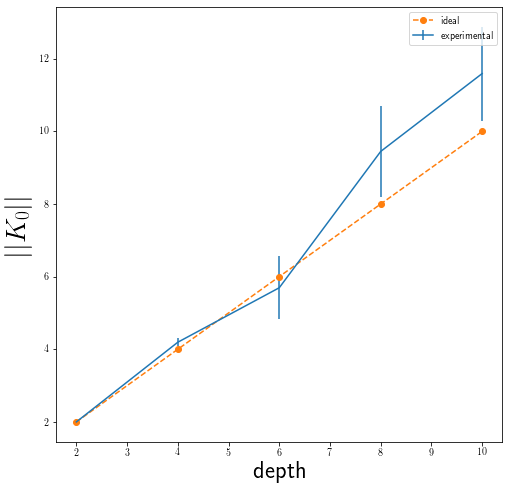
\includegraphics[scale=0.4]{figs/dln-k-vs-d.png}
&
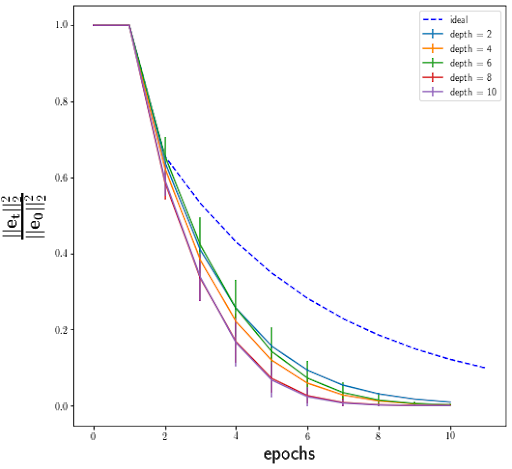
\includegraphics[scale=0.4]{figs/dln-conv.png}
&
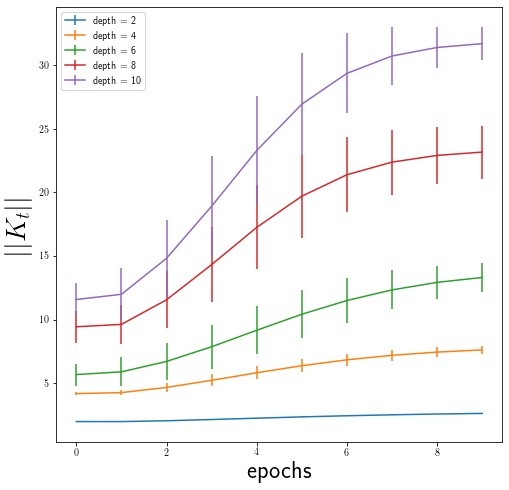
\includegraphics[scale=0.4]{figs/dln-gram.png}
&
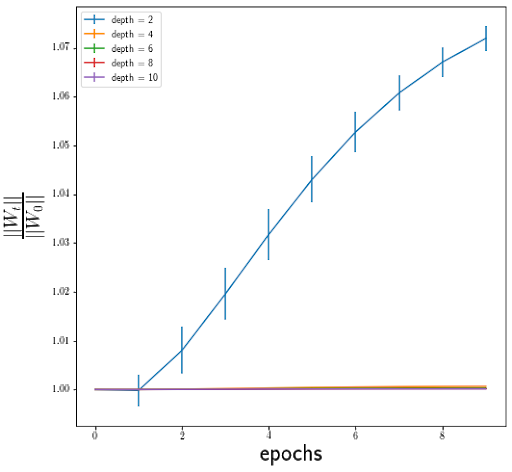
\includegraphics[scale=0.4]{figs/dln-norm.png}
\end{tabular}
}
\caption{In all the plots $d_{in}=1, n=1, w=100,\sigma^2=\frac{1}{w}$ averaged over $5$ runs. The left most plot shows $K_0$ as a function of depth. The second from left plot shows the convergence rate. The third plot from left shows the growth of $K_t$ over the course of training, and the right most plot shows the growth of weights ($L_2$-norm) with respect to time.}
\label{fig:dln}
\end{figure*}

\comment{\section{DGN-FRG}
\textbf{Effect of $p$} is shown in \Cref{fig:peff}. For $w=100$, we observe that for  the e.c.d.f gets better as the value of $p$ reduces till $p=0.3$, after which it starts degrading. This is due to the fact that the variance gets worse with $\frac{1}p$ (since $\sigma=\sqrt{\frac{1}{pw}}$. It can be seen that for $w=50$ the variance is more and hence the e.c.d.f gets better as we reduce $p$ only till $p=0.4$, after which it starts to degrade.

\FloatBarrier
\begin{figure*}[h]
\resizebox{\columnwidth}{!}{
\begin{tabular}{cc}
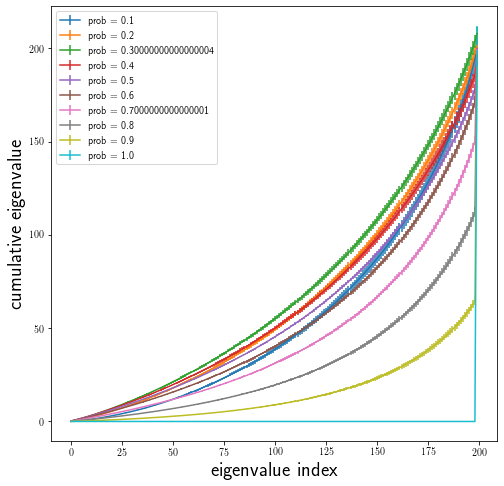
\includegraphics[scale=0.4]{figs/dgn-frg-ecdf-p-w100.png}
&
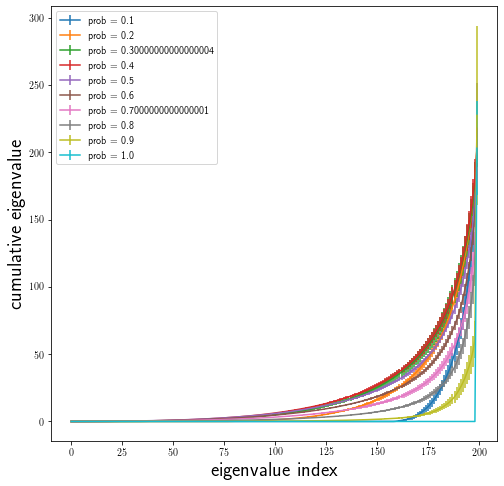
\includegraphics[scale=0.4]{figs/dgn-frg-ecdf-p-w10.png}
\end{tabular}
}
\caption{Shows e.c.d.f for various values of $p$.}
\label{fig:peff}
\end{figure*}}


\textbf{Statement and Proof of Lemma~\ref{lm:invariance}}
\begin{lemma}
At $t=0$, under Assumptions~\ref{assmp:mainone},\ref{assmp:maintwo}, convolutional layers with global average pooling at the end causes translational invariance.
\begin{align*}
&\E{x_s(L,1)x_{s'}(L,1)}\\&=\frac{\sigma^{2(d-1)}}{d^2_{in}}\sum_{k=1}^{\hat{B}} \sum_{p_1,p_2\in b_k}  \Big( x(p_1(0),s) A(x_s,p_1)\\
&\quad\quad \quad\quad \quad\quad x(p_2(0),s') A(x_{s'},p_2) \Big)
\end{align*}
\end{lemma}

\begin{proof}
\begin{align*}
\E{x_s(L,1)x_{s'}(L,1)}&=\E{\phi^\top_{x_s,\G_0} w_0w_0^\top \phi^\top_{x_{s'},\G_0}}\\
&=\phi^\top_{x_s,\G_0}\E{ w_0 w_0^\top} \phi^\top_{x_{s'},\G_0},
\end{align*}
where we use the fact that the gates $\G_0$ are statistically independent of the weights. Now let $M=\E{ w_0 w_0^\top}$, we make the following observations about $M$:

$1.$ $M(p_1,p_2)=0$, if $p_1$ and $p_2$ belong to the different bundles.

$2.$ $M(p_1,p_2)=\frac{\sigma^{2(d-1)}}{d^2_{in}}$, if $p_1$ and $p_2$ belong to the same bundle.

Using the above two observations, we have at  $t=0$:

\begin{align*}
&\E{x_s(L,1)x_{s'}(L,1)}\\&=\phi^\top_{x_s,\G_0} M \phi^\top_{x_{s'},\G_0}\\
&=\sum_{p_1,p_2=1}^{\hat{P}} \Big(x(p_1(0),s) A(x_s,p_1) \\
&\quad\quad \quad\quad \quad\quad x(p_2(0),s') A(x_{s'},p_2) M(p_1,p_2)\Big)\\
&=\frac{\sigma^{2(d-1)}}{d^2_{in}}\sum_{k=1}^{\hat{B}} \sum_{p_1,p_2\in b_k}  \Big( x(p_1(0),s) A(x_s,p_1)\\
&\quad\quad \quad\quad \quad\quad x(p_2(0),s') A(x_{s'},p_2) \Big)
\end{align*}
\end{proof}


